\chapter{Problématique et organisation}
\section{LaBRI et SCRIME}
Le stage s'est déroulé du deux février au treize juin, dans les bâtiments du \ac{SCRIME} et en tant que stagiaire du \ac{LaBRI}. L'équipe dont je fais partie est variable mais j'étais entouré de deux ingénieurs affectés à ce projet, ainsi que plusieurs autres stagiaires.

J'ai rencontré mes tuteurs, Mme. Desainte-Catherine et M. Chaumette, de manière très régulière, quasiment chaque semaine, pour faire un point sur mon avancement.

\section{Projet OSSIA}
Le stage s'inscrit dans le cadre du projet \brand{ANR} \ac{OSSIA}. Ce projet, démarré en 2012, apporte une réponse aux questions posées lors du projet \brand{ANR Virage}, qui avait pour but de dresser un état des lieux des besoins et pratiques en terme de contrôle et d'écriture dans le cas des contenus en temps réel, puis d'établir un cahier des charges pour une solution unificatrice pour la conception de scénarios, et l'écriture du temps dans un cadre intermédia.

Ainsi, \ac{OSSIA} conçoit un formalisme et un cadre logiciel correspondant à ces attentes.

Des acteurs d'origines diverses participent au projet:
\begin{itemize}
	\item Des laboratoires : \ac{LaBRI}, \ac{GMEA}.
	\item Une école : \ac{ENJMIN}.
	\item Des sociétés : \brand{Blue Yeti}, \brand{RSF}.
	\item Des artistes : \brand{Les Baltazars}, \brand{Renaud Rubiano}.
	\item Des développeurs.
\end{itemize}

Les interactions parfois complexes entre ces acteurs sont expliquées dans \cite{meyssonnier2013analyse}.

\subsection{Formalisme}
Les travaux du projet portent en partie sur la réalisation d'un formalisme assez expressif pour permettre de s'en servir dans des cas d'usages très différents.

Ce formalisme repose sur la notion de scénario interactif, qui elle-même repose sur la notion de temps, au sens ou on l'entend couramment, mais aussi étendu des manières suivantes :
\begin{table}[H]
	\centering
	\tabulinesep=3pt
	\begin{tabu} to \linewidth {XX[4]}
		Type de temps 	& Définition \\	\toprule[0.15em]
		Souple			& Temps géré par une horloge dont la fréquence peut être contrôlée par un facteur multiplicatif \\ \midrule
	
		Conditionnel	& Activation ou non de certaines parties en fonction d'un évènement extérieur\\ \midrule
		Non-linéaire	& Bouclage, reprise, dédoublement\dots \\ \midrule
		Hiérarchique	& Permet une meilleure organisation et la présence de sous-temps. \\ 
	\end{tabu}
	\caption{Les différentes familles de temps considérés dans \brand{OSSIA}}
\end{table}

\begin{mydef}[Scénario] Une structure pouvant contenir du temps.
\end{mydef}

Néanmoins, le temps seul n'est pas utile : il faut qu'il y ait une notion de contrôle d'éléments extérieurs, comme par exemple le volume d'un fichier audio, ou l'intensité d'un éclairage.

Ce contrôle se fait au travers de la notion de processus.

\begin{mydef}[Processus] Le changement d'un paramètre au cours du temps.
\end{mydef}

Des exemples de scénarios et de processus sont visibles dans les captures d'écrans de la \cref{figIScore}.

\subsection{Logiciel i-score}
Le logiciel i-score est en développement depuis plusieurs années, et comporte l'héritage de plusieurs autres logiciels et paradigmes qui ont été développé avant lui, comme visible en \cref{figheritageIScore}.

\begin{figure}[H]
	\centering
	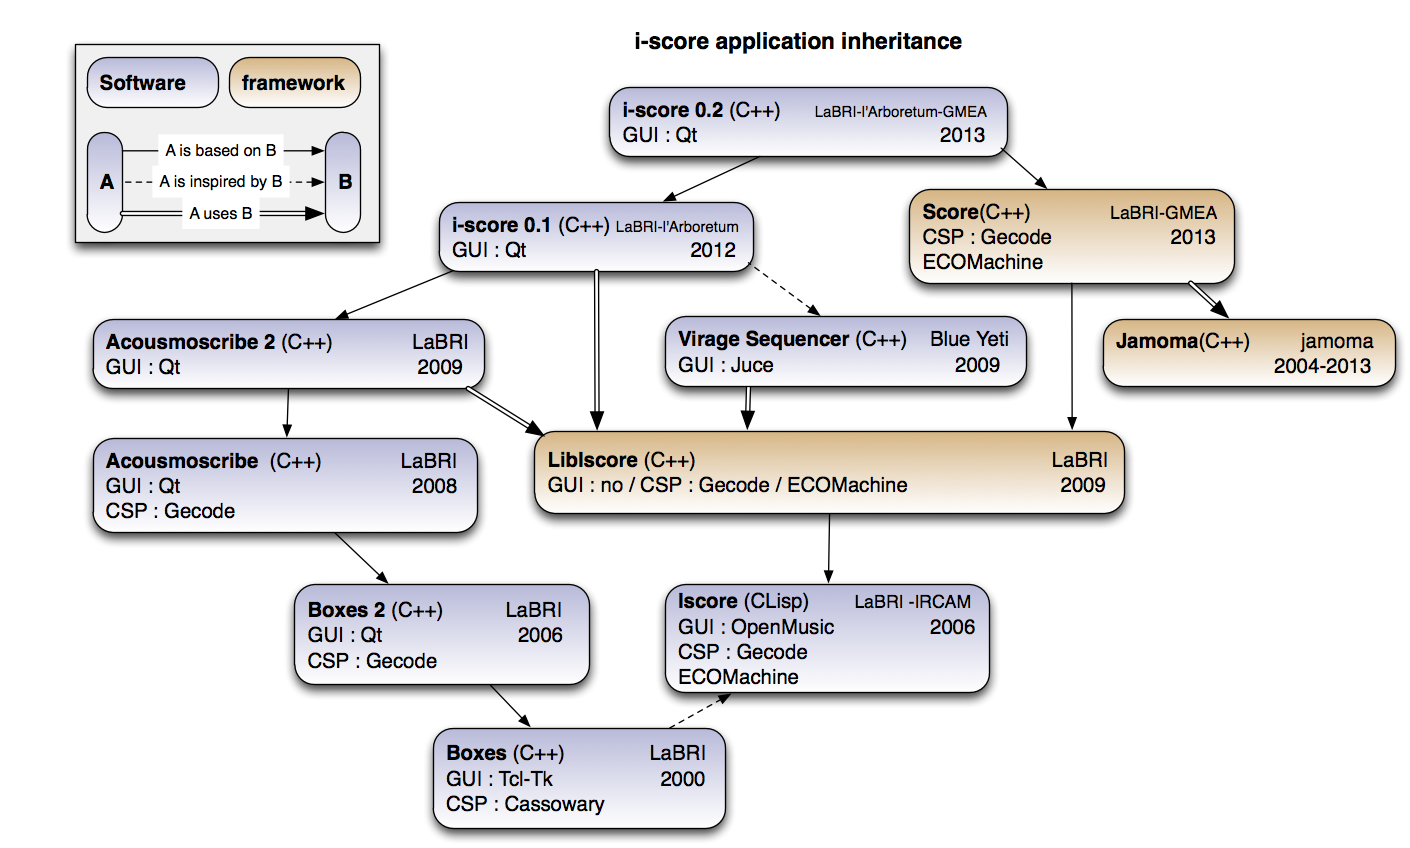
\includegraphics[scale=0.4]{images/iscoreHeritage.png}
	\caption{Les racines du logiciel i-score}
	\label{figheritageIScore}
\end{figure}

Actuellement, il incarne à la fois l'outil permettant d'écrire les scénarios, et de les exécuter.

Deux versions d'i-score (captures d'écran en \cref{figIScore}) sont en développement parallèle : i-score 0.2, une version fonctionnelle mais qui n'inclut pas les travaux les plus récents du paradigme \ac{OSSIA}, et i-score 0.3, une version pour l'instant non-fonctionnelle, mais qui a pour vocation de représenter l'état actuel du développement théorique.

\begin{figure}[H]
	\centering
	\begin{subfigure}{.5\textwidth}
		\centering
		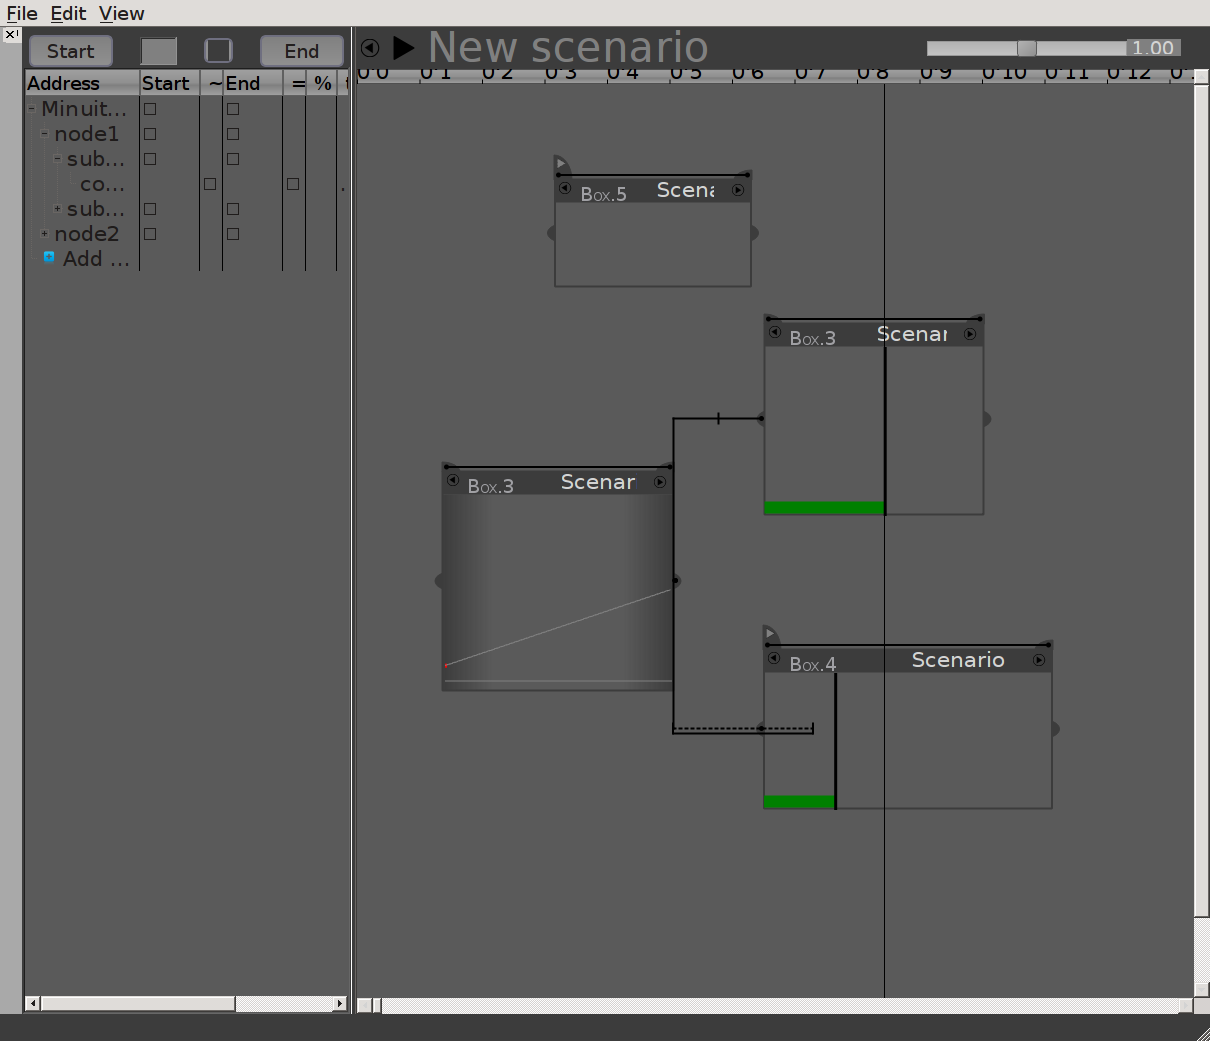
\includegraphics[scale=0.2]{images/iscore02.png}
		\caption{Version 0.2}
	\end{subfigure} 
	
	\vspace{1em}
	
	\begin{subfigure}{.5\textwidth}
		\centering
		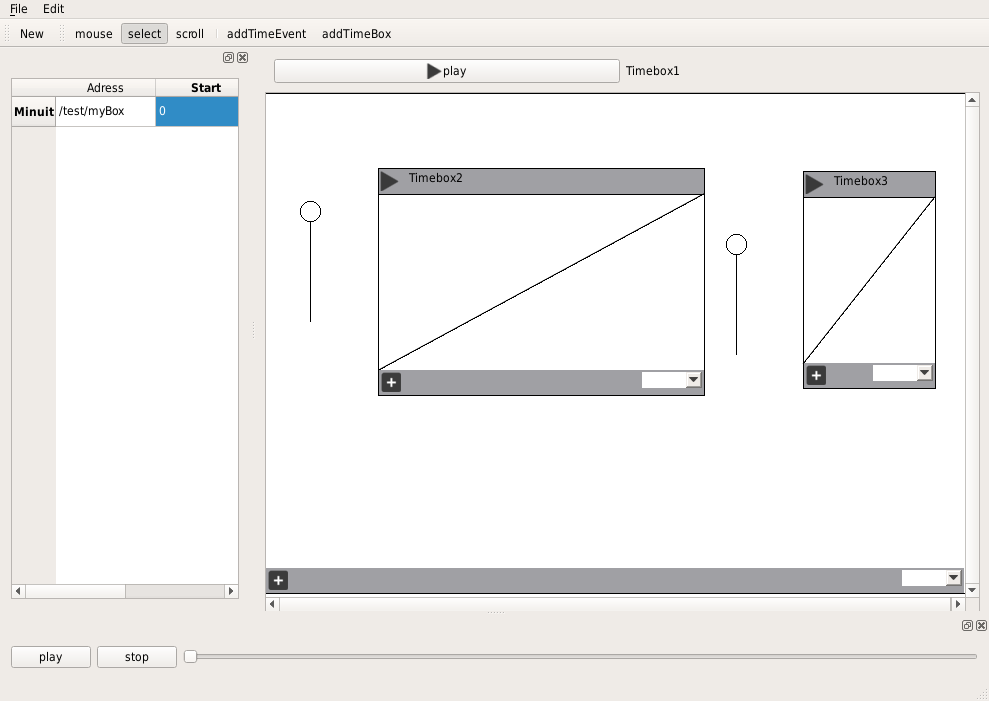
\includegraphics[scale=0.2]{images/iscore03.png}
		\caption{Version 0.3}
	\end{subfigure}
	
	\caption{Captures d'écran des deux version d'i-score.}
	\label{figIScore}
\end{figure}

\subsection{Score et API OSSIA}
\subsubsection{Score}
Score est la bibliothèque sous-jacente qui comporte la logique utilisée pour faire l'exécution d'i-score. Elle contient différents moteurs :

\begin{itemize}
	\item Un moteur d'exécution à base de réseaux de Petri.
	\item Un résolveur de \ac{CSP}, utilisé pour l'édition et plus spécifiquement le déplacement des boîtes.
\end{itemize}

Cette bibliothèque utilise le cadriciel \brand{Jamoma}.

\subsubsection{API}
La version 0.3 d'i-score se base sur une \ac{API}, qui offre toutes les possibilités de gestion de scénario directement au programmeur, de manière à ce que d'autres applications puissent être conçues par dessus. Par exemple, des acteurs du jeu vidéo sont intéressés par le fonctionnement offert par \ac{OSSIA} dans un environnement \brand{Unity}. 

\section{Répartition et attentes}
\subsection{Problèmes posés par la répartition}
Un des problèmes majeurs ici est le besoin de synchronisation avec une horloge physique. En effet, les relations entre débuts et fins d'évènements sont données sous forme de millisecondes les séparant, les réseaux étant temporels. Ainsi, les mécanismes d'horloges vectorielles et logiques ne sont pas directement applicables.

Le deuxième problème est qu'il n'est pas réellement question de répartition au sens couramment entendu dans le domaine de l'informatique répartie. En effet, ici, les processus correspondent à des besoins physiquement présents sur des machines et qui ne peuvent pas être déplacés sur d'autres machines. Par exemple, une machine peut avoir une sortie vidéo, et une autre machine une carte son : cela conditionne pour le compositeur l'endroit ou s'exécute un processus, selon qu'il soit relatif à l'image ou au son.

Idéalement, il serait possible de faire une différenciation automatique, néanmoins, deux aspects s'y opposent : 
\begin{itemize}
\item Le compositeur désire avoir le choix pour la répartition.
\item Score ne communique qu'avec des messages \ac{OSC}. Un message \ac{OSC} a le format suivant : 
\begin{verbatim} /adresse/où/écrire argument1 argument2 ... \end{verbatim}.

Les adresses sont laissées à la discrétion des logiciels avec lesquels Score communique, car non standardisées. Il n'est donc pas possible de savoir quel type d'information est communiqué. 
\end{itemize}
Un troisième point, limitant, à tenir en compte, est celui de la gestion de l'interactivité. Dans ce cas, l'impact de la latence due au réseau physique est inévitable.

\section{Organisation au cours du stage}
Cette partie précisera le déroulement de mon stage : compréhension du sujet, recherche, implémentation\dots

Pour rappel, le sujet précis du stage était : 
\begin{center}
	\noindent\fbox{\parbox{31em}{Répartition du séquenceur multimedia i-score sur plusieurs machines.}}
\end{center}


\subsection{Définition du travail à réaliser}
\subsection{Organisation temporelle}
(TODO mettre diagramme de Gantt)